\chapter{Cross Section Determination Method}
\label{crosssectionchapter}
\label{limits}

This chapter summarizes the technique used to measure the single top quark cross section as well as the systematic uncertainties on the expected signal and background yields. Section~\ref{CrossSectionDetermination} derives the Bayesian posterior density function and shows how it is used to determine the single top quark production cross section. The treatment of systematic uncertainties is also covered in this section. A description of each systematic uncertainty and its effect on the signal acceptance and background yield is presented in Section~\ref{systematics}. Section~\ref{ensembles} describes the method designed to measure the stability and linearity of the cross section measurement technique. Finally, the expected sensitivity and cross section resolution for a Standard Model single top signal in the full dataset is presented in Section~\ref{exp-performance}.

\section{Bayesian Posterior Density Function}
\label{CrossSectionDetermination}

The single top cross section is measured by creating a Bayesian posterior density function, which yields the probability density for all single top quark production cross sections\footnote{The Bayesian posterior density function is sometimes referred to as the posterior in this text.}. The posterior is defined as the conditional probability that a process $\mathcal{A}$ is true given that another process $\mathcal{B}$ is also true; it is equal to the conditional probability of process $\mathcal{B}$ given process $\mathcal{A}$ multiplied by the prior probability for process $\mathcal{A}$ ($\pi(\mathcal{A})$) divided by the prior probability for process $\mathcal{B}$ ($\pi(\mathcal{B})$), as shown in  Eq.~\ref{bayestheorem}.

\begin{equation}
\label{bayestheorem}
P(\mathcal{A}|\mathcal{B}) = \frac{P(\mathcal{B}|\mathcal{A})\pi(\mathcal{A})}{\pi(\mathcal{B})}
\end{equation}

In the single top quark analysis $\mathcal{A}$ is the number of signal and background events and $\mathcal{B}$ is the observed number of events. The conditional probability $P(\mathcal{B}|\mathcal{A})$ is then interpreted as the probability to observe $N$ events given $n$, where $n$ is the expected number of signal and background events. Numerically this is given as the value of the Poisson probability density function for observed number of events given the expectation as seen in Eq.~\ref{poisson}. This term is also referred to as the likelihood and its application in the single top quark analysis is given latter in this section.

\begin{equation}
\label{poisson}
P(\mathcal{B}|\mathcal{A}) \equiv \mathcal{L}(N|n) = \frac{n^{N}e^{-n}}{N!}
\end{equation}

The quantity of interest in this analysis is the signal cross section and not the number of expected signal and background events. To expose the cross section dependence the expected yield $n$ is re-written as

\begin{equation}
\label{expected}
n = n_{S} + n_{B} = \alpha_{S} L \sigma_{S} + \sum_{i} n_{B,i},
\end{equation}

\noindent where $\alpha_{S}$ is the signal acceptance, $L$~is the integrated luminosity, $\sigma_{S}$ is the signal cross section, and $\sum_{i} n_{B,i}$ is the sum of background yields.\footnote{For the rest of this section, the luminosity is absorbed by the acceptance term ($\alpha_{S} \times L \rightarrow \alpha_{S}$).} The likelihood is also re-written as $\mathcal{L}(N|n) = \mathcal{L}(N|\sigma_{S},\alpha_{S},\vec{n}_{B})$ and the prior $\pi(n)$ is re-written as $\pi(\sigma_{S},\alpha_{S}, \vec{n}_{B})$. 

The prior can be factored into a term dependent on the cross section and a term dependent on the signal acceptance and the background yield as shown in Eq.~\ref{prior}. 

\begin{equation}
\label{prior}
\pi(n) \equiv \pi(\sigma_{S},\alpha_{S}, \vec{n}_{B}) = \pi(\sigma_{S}) \times \pi(\alpha_{S}, \vec{n}_{B})
\end{equation}

The likelihood is modified to combined multiple independent channels by replacing the original likelihood by the product of the likelihoods for each channel, as shown in Eq.~\ref{combine}.

\begin{equation}
\label{combine}
\mathcal{L}(N|\sigma_{S},\alpha_{S}, \vec{n}_{B}) \rightarrow \prod_{i} \mathcal{L}(N_{i}|\sigma_{S},\alpha_{S,i}, \vec{n}_{B,i})
\end{equation}

For the matrix element analysis method the values of $N$,~$\alpha$, and~$\vec{n}_{B}$ are given in the form of two-dimensional histograms, where one axis corresponds to the $s$-channel discriminant and the other axis corresponds to the $t$-channel discriminant. The histograms are filled with matrix element discriminants for the data (N), the signal Monte Carlo ($\alpha_{S}=n_{S}/\sigma_{S}$), and background Monte Carlo ($\vec{n}_{B}$). To incorporate the shape information of these quantities, the likelihood is further modified for a given channel as the product of the likelihoods for each bin in the two-dimensional histogram, as shown in Eq.~\ref{bins}.

\begin{equation}
\label{bins}
\mathcal{L}(N|\sigma_{S},\alpha_{S}, \vec{n}_{B}) \rightarrow \prod_{\rm{Bins}\{j\}} \mathcal{L}(N_{j}|\sigma_{S},\alpha_{S,j}, \vec{n}_{B,j})
\end{equation}

The acceptance and background yield dependence on the posterior are removed by integrating the likelihood and prior with respect to the signal acceptance and each background yield, as shown in Eq.~\ref{remove}.

\begin{equation}
\label{remove}
P(\sigma|N) = \frac{1}{P(N)} \int \int \mathcal{L}(N|\sigma_{S},\alpha^{'}_{S}, \vec{n}^{'}_{B}) \times \pi(\sigma_{S}) \times \pi(\alpha^{'}_{S}, \vec{n}^{'}_{B}) ~ d\alpha^{'}_{S} d\vec{n}^{'}_{B}
\end{equation}

\noindent The term $P(N)$ is the posterior normalization such that the posterior retains a probability density function interpretation (i.e~$\int P(\sigma|N) \rm{d}\sigma = 1$~). To ensure that the normalization is finite the prior for the signal cross section $\pi(\sigma_{S})$ is cut off at a maximum value, $\sigma_{\rm{max}}$. The prior is flat in the region of $0<\sigma<\sigma_{\rm{max}}$ and zero beyond this region.\footnote{A flat prior represents a minimal bias towards any signal cross section.} The value of $\sigma_{\rm{max}}$ is chosen to be large enough such that beyond that limit the likelihood is negligibly small for all $\alpha_{S}$ and $\vec{n}_{B}$.

The prior $\pi(\alpha^{'}_{S}, \vec{n}^{'}_{B})$ is defined separately for the case of no systematics uncertainties and complete systematics. Both cases are described in the following section.

\subsection{Prior Definition With and Without Systematic Uncertainties}

\subsubsection{Prior Without Systematics}

In the case of no systematic uncertainties the signal acceptance and background yields are perfectly known. This requires the prior to be a product of two delta functions, as shown in Eq.~\ref{priornosys}, and leads to a posterior shown in Eq.~\ref{postnosys}.

\begin{equation}
\label{priornosys}
\pi(\alpha^{'}_{S}, \vec{n}^{'}_{B})=\delta(\alpha^{'}_{S}-\alpha_{S})\times\delta(\vec{n}^{'}_{B}-\vec{n}_{B})
\end{equation}

\begin{equation}
\label{postnosys}
P(\sigma|N) = \frac{\mathcal{L}(N|\sigma_{S},\alpha_{S}, \vec{n}_{B}) \times \pi(\sigma_{S})}{\int \mathcal{L}(N|\sigma^{'}_{S},\alpha_{S}, \vec{n}_{B}) \times \pi(\sigma^{'}_{S})~d\sigma^{'}_{S}}
\end{equation}

\subsubsection{Prior With Systematics}

In the case of systematic uncertainties the prior is modified to reflect the uncertainty in $\alpha_{S}$ and $\vec{n}_{B}$. For each systematic uncertainty the $\pm$1$\sigma$~uncertainty is propagated through the analysis resulting in a $\pm$1$\sigma$~uncertainties for the signal acceptance~($\delta\alpha_{S}$) and the background yield~($\delta\vec{n}_{B}$). From these values a covariance matrix is created, which accounts for all correlations between systematics (e.g. the uncertainty in the integrated luminosity affects both the signal acceptance and the $\ttbar$ normalization). The covariance matrix element \{i,j\} for background or signal $i$ and $j$ is defined as

\begin{equation}
\rm{cov}_{i,j} = p_{i}p_{j} \sum_{k=1}^{m} f_{i,k}f_{j,k},
\end{equation}

\noindent where $p_{i}$ is the signal or background yield for the $i^{th}$ source and $f_{i,k}$ is the fractional uncertainty from the $k^{th}$ systematic component for the $i^{th}$ signal or background. The prior is then calculated as a multivariate Gaussian, as shown in Eq.~\ref{priorsys}.

\begin{equation}
\label{priorsys}
\pi(\alpha^{'}_{S}, \vec{n}^{'}_{B})= \frac{1}{\sqrt{(2\pi)^{N}|\Sigma|}} \mathrm{exp} \left\{ -\frac{1}{2}(\vec{x} - \mu)^{T} \Sigma^{-1} (\vec{x}-\mu) \right\}
\end{equation}

\noindent where $\Sigma$ is the covariance matrix, $\vec{x}$ represents $\{ \alpha^{'}_{S}, \vec{n}^{'}_{B} \}$, and $\mu$ represents $\{ \alpha_{S}, \vec{n}_{B} \}$

The posterior, when systematics are included, is solved using Monte Carlo importance sampling. In this method a set of points in $\{ \alpha_{S}, \vec{n}_{B} \}$-space are generated according the prior density defined in Eq.~\ref{priorsys}. The solution to the posterior is given by

\begin{equation}
\label{mcint}
\int \int \mathcal{L}(N|\sigma_{S},\alpha_{S}, \vec{n}_{B}) \times \pi(\alpha_{S}, \vec{n}_{B}) ~ d\alpha_{S}d\vec{n}_{B} = \frac{1}{K} \sum_{i=1}^{K} \mathcal{L}(N|\sigma_{S},\alpha_{S}, \vec{n}_{B})
\end{equation}

A discussion of the systematic uncertainties and their magnitudes can be found in Section~\ref{systematics} of this chapter.

\subsection{Cross Section Extraction}

If there is an excess of data events over the expected background yield then it is possible to determine the production cross section for a given process. The cross section is defined as the value which maximizes the posterior, as seen in Fig.~\ref{CrossSection}. The solid blue line represents the cross section (3.9 pb) and the dashed-blue lines represent the $\pm1\sigma$ uncertainty on the cross section. The uncertainties are calculated by integrating the posterior curve until 33.15$\%$ of the area is contained on each side of the cross section. In the case of Fig.~\ref{CrossSection} the $+1\sigma$ error band covers 2.3~pb above the cross section and the $-1\sigma$ error band covers 2.2~pb below the cross section.

\begin{figure}[!h!tbp]
\begin{center}
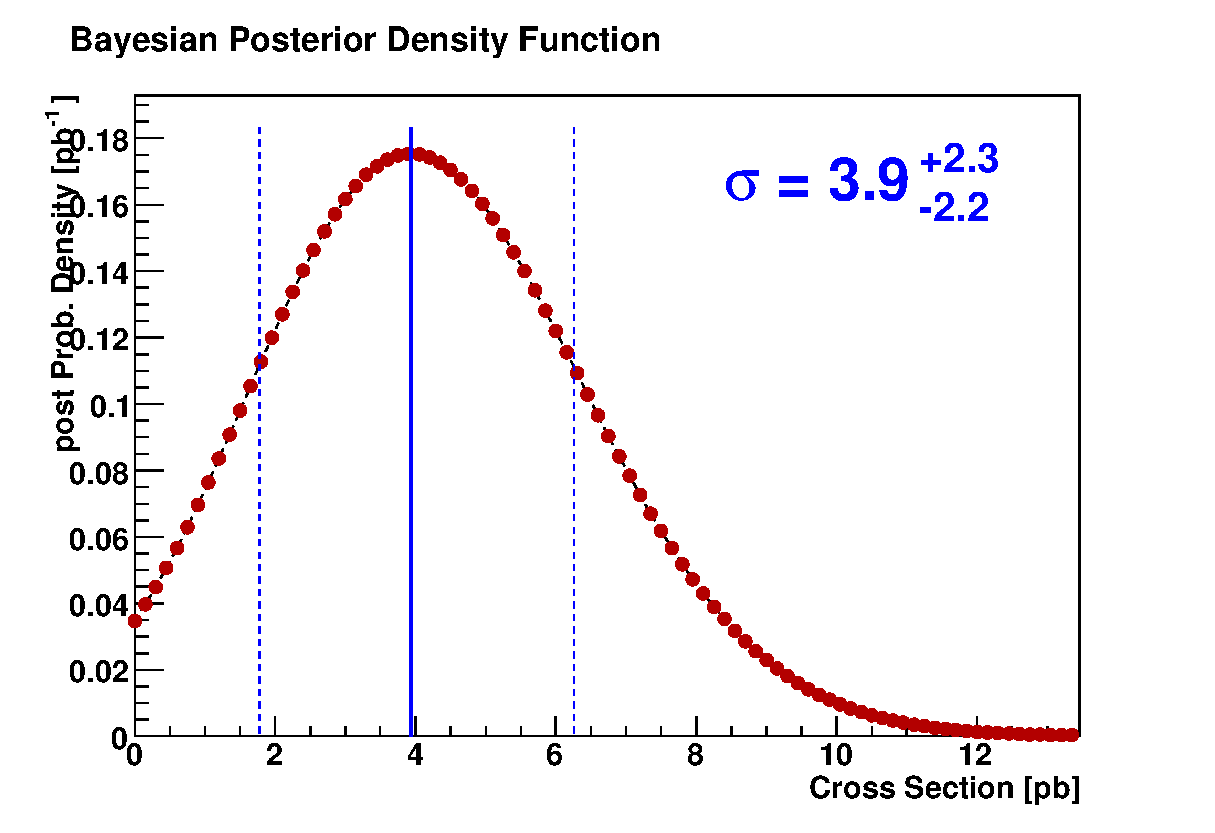
\includegraphics[width=0.75\textwidth]{eps/Limits/CrossSection.eps}
\end{center}
\vspace{-0.1in}
\caption{Example cross section measurement (solid blue line) with $\pm1\sigma$ error band (dashed blue lines).}
\label{CrossSection}
\end{figure}

If there is no excess of data above the background, then upper limits on the production cross section can be set. An upper cross section limit, $\sigma_{\rm{CL}}$, at a given confidence level is found by integrating the posterior until an area equal to the confidence level is obtained, as shown in Eq.~\ref{cl}. Fig.~\ref{CrossSectionLimit} shows the cross section limit for the same posterior shown in Fig.~\ref{CrossSection}. The limit is 8.4 pb at 95$\%$~CL.

\begin{equation}
\label{cl}
\int_{0}^{\sigma_{\rm{CL}}} P(\sigma|N)~d\sigma = CL
\end{equation}



\begin{figure}[!h!tbp]
\begin{center}
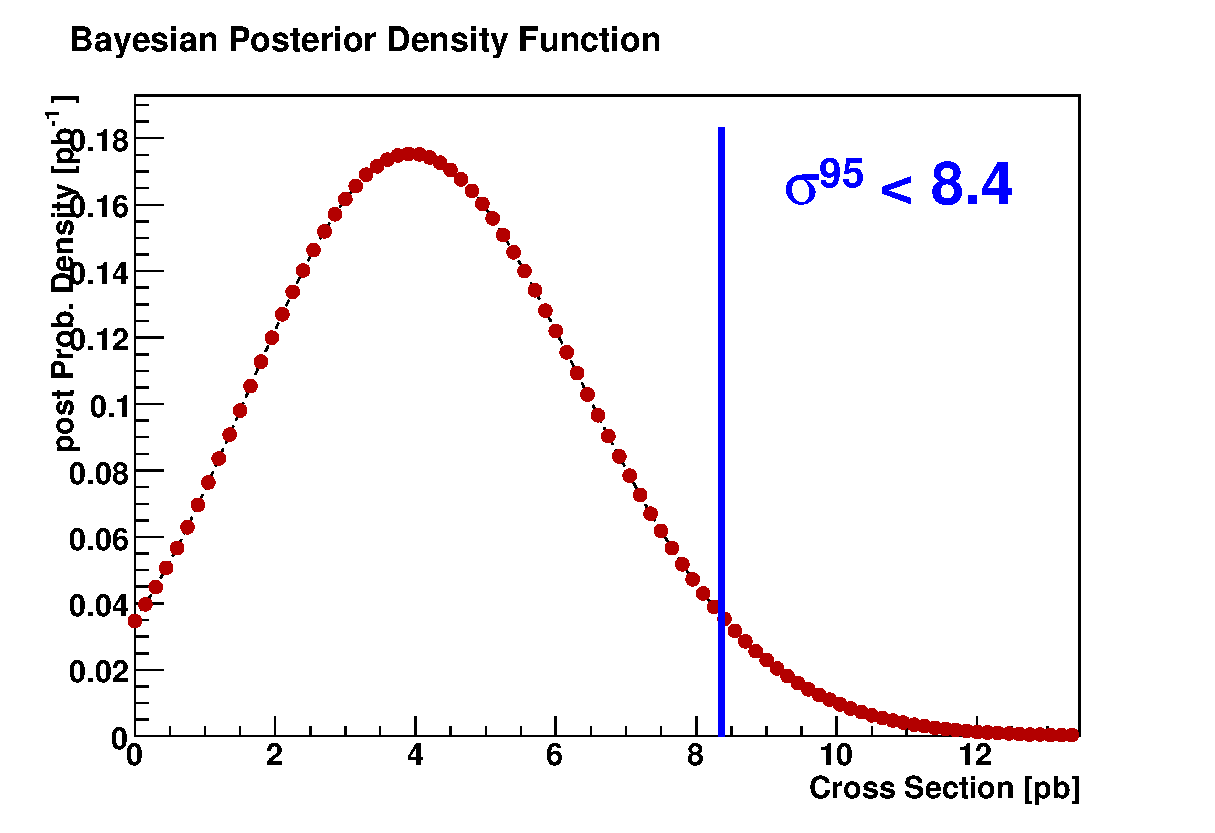
\includegraphics[width=0.75\textwidth]{eps/Limits/Limit.eps}
\end{center}
\vspace{-0.1in}
\caption{Example of the 95$\%$~CL upper cross section limit. The value of the upper limit is shown by the blue curve. For this posterior the cross section limit is 8.4 pb.}
\label{CrossSectionLimit}
\end{figure}

Finally, a quantity used to optimize the sensitivity of a particular analysis channel is the Bayes ratio. This quantity is an approximation to the Bayes factor which is the likelihood for the case of signal+background divided by the background only likelihood. The Bayes ratio is defined as the ratio of the posterior at its maximum over the posterior at zero cross section. The larger the Bayes ratio the more sensitive a channel is to measure a cross section different from zero. This is shown graphically in Fig.~\ref{BayesRatio} for the same posterior curve used in the previous two figures.

\begin{figure}[!h!tbp]
\begin{center}
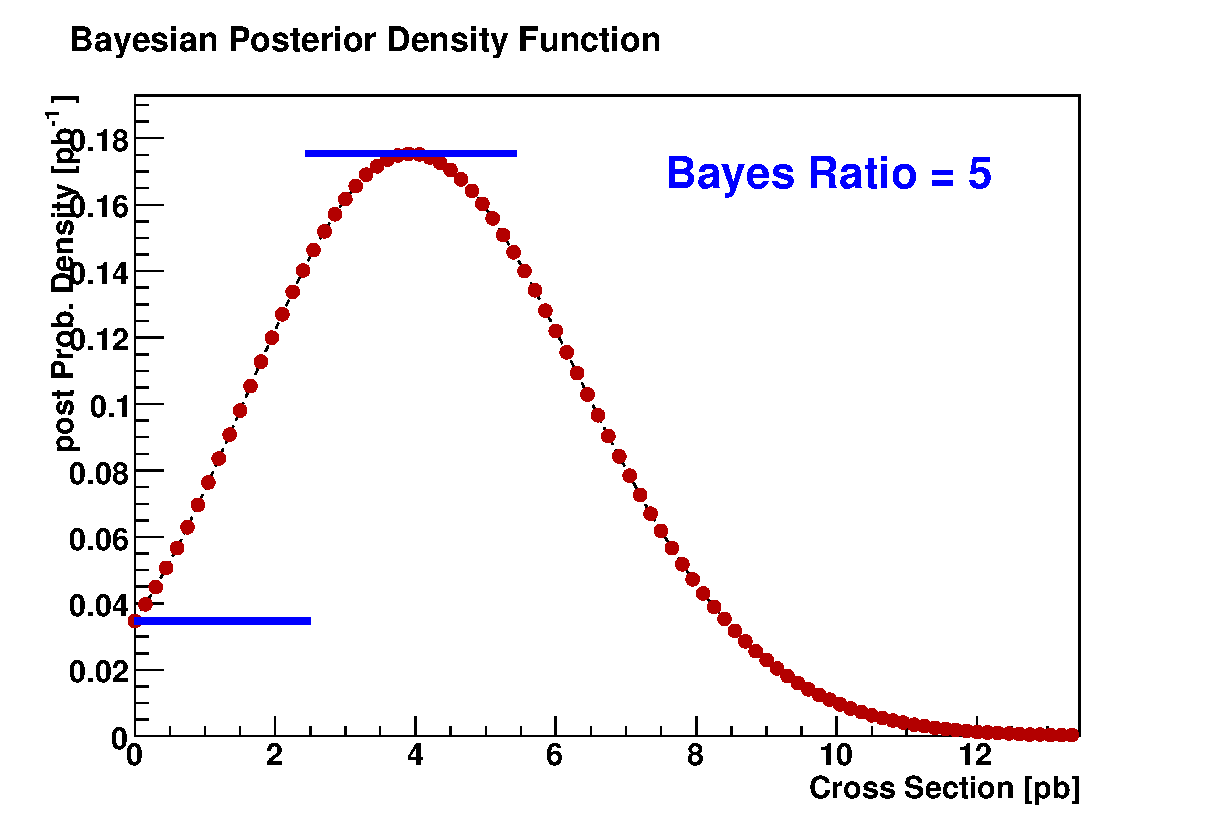
\includegraphics[width=0.75\textwidth]{eps/Limits/BayesRatio.eps}
\end{center}
\vspace{-0.1in}
\caption{Example of the Bayes ratio defined as the maximum of the posterior (top blue line) over the posterior at zero cross section (lower blue line). The Bayes ratio for this curve is 5.0.}
\label{BayesRatio}
\end{figure}

\subsection{$s+t$-channel Cross Section Definition}

All cross sections presented in this thesis are the combined $s$-channel plus $t$-channel cross section. In this case the ratio of $s/t$-channel cross sections ($0.88/1.98=0.44$) is assumed to be consistent with the Standard Model. With an increased dataset a measurement of the individual $s$-channel and $t$-channel cross sections will be a future addition to this analysis.

\clearpage
\section{Systematic Uncertainties}
\label{systematics}
\label{sysdescription}

This section describes all systematic uncertainties considered in the matrix element analysis. In most cases the uncertainty source applies both to the signal acceptance ($\alpha$) and the background expectation ($n_{B}$). The other systematics are only applied to certain backgrounds as explained in the following text. Two sources of systematic uncertainties (jet energy scale and tag-rate functions) are referred to as  ``shape changing'' systematics, while the rest solely affect the signal or background normalization and are referred to as ``flat'' systematics. Flat systematics have a uniform uncertainty across all bins of the matrix element discriminant, while shape changing systematics vary bin-to-bin. Table~\ref{tab:generalsys} summarizes the relative uncertainties due to each systematic source\footnote{Appendix~\ref{allsys}~shows the uncertainties for each background yield and signal acceptance for each analysis channel.}. The effect of each systematic uncertainty on the measured single top cross section can be found in Chapter~\ref{results}.

\vspace{-0.1in}
\begin{table}[h]
\begin{center}
\caption{A summary of the relative systematic uncertainties
for each of the applied corrections and efficiencies. The uncertainty
shown is the error on the correction or the efficiency, before it has
been applied to the MC or data samples.}
\label{tab:generalsys}
\begin{tabular}{c|c||c|c}
%\multicolumn{4}{c}{\underline{Relative Systematic Uncertainties}}\\
\hline
{\ttbar} cross section		& $18\%$		& Primary vertex                    			&  $3\%$  \\
Luminosity                      	&  $6\%$  		& Electron reco * ID                			&  $2\%$  \\
Electron trigger                   & $3\%$   		& Electron trackmatch \& likelihood 		&  $5\%$  \\
Muon trigger                       	& $6\%$   		& Muon reco * ID                    			&  $7\%$  \\
Jet energy scale               	&wide range	& Muon trackmatch \& isolation      		&  $2\%$  \\
Jet efficiency                     	& $2\%$  		& Electron~$\varepsilon_{\rm{W+jets}}$ 	&  $2\%$  \\
Jet fragmentation              	& 5--7$\%$	& Muon~$\varepsilon_{\rm{W+jets}}$    	&  $2\%$  \\
Heavy flavor ratio             	& $30\%$  	& Electron~$\varepsilon_{\rm{Multijet}}$ 	&3--40$\%$\\ 
Tag-rate functions             	&2--16$\%$	& Muon~$\varepsilon_{\rm{Multijet}}$    	&2--15$\%$
\end{tabular}
\end{center}
\end{table}


\begin{itemize}
\item {\bf Integrated luminosity} \\ 
The error on the integrated luminosity used in the analysis is $6.1\%$. This uncertainty comes from the error on the measured inelastic $\ppbar$~cross section. The error on the luminosity estimate affects the $\ttbar$ background since this background is normalized using the integrated luminosity.

\item {\bf Theoretical cross sections} \\ 
The $\ttbar$ background yield is normalized to the NLLO theoretical cross section. The uncertainty of this cross section for a top mass of 175~GeV is $18\%$. The uncertainty on the cross section is mainly due to the uncertainty from the top mass, but also from the choice of scale and parton distribution function uncertainties.

\item {\bf Trigger efficiency} \\
The uncertainty on the trigger efficiency is determined by varying the trigger term efficiencies at each trigger level by the $\pm1\sigma$ uncertainties. A total uncertainties of $3\%$ was assigned to the $e$+jets trigger and $6\%$ to the $\mu$+jets trigger. Fig.~\ref{triggeruncer} shows the affect of the $\pm1\sigma$~shift in the $e$+jets trigger efficiency on the electron $p_{T}$ in $\dilepton$ Monte Carlo events.

\begin{figure}[!h!tbp]
\begin{center}
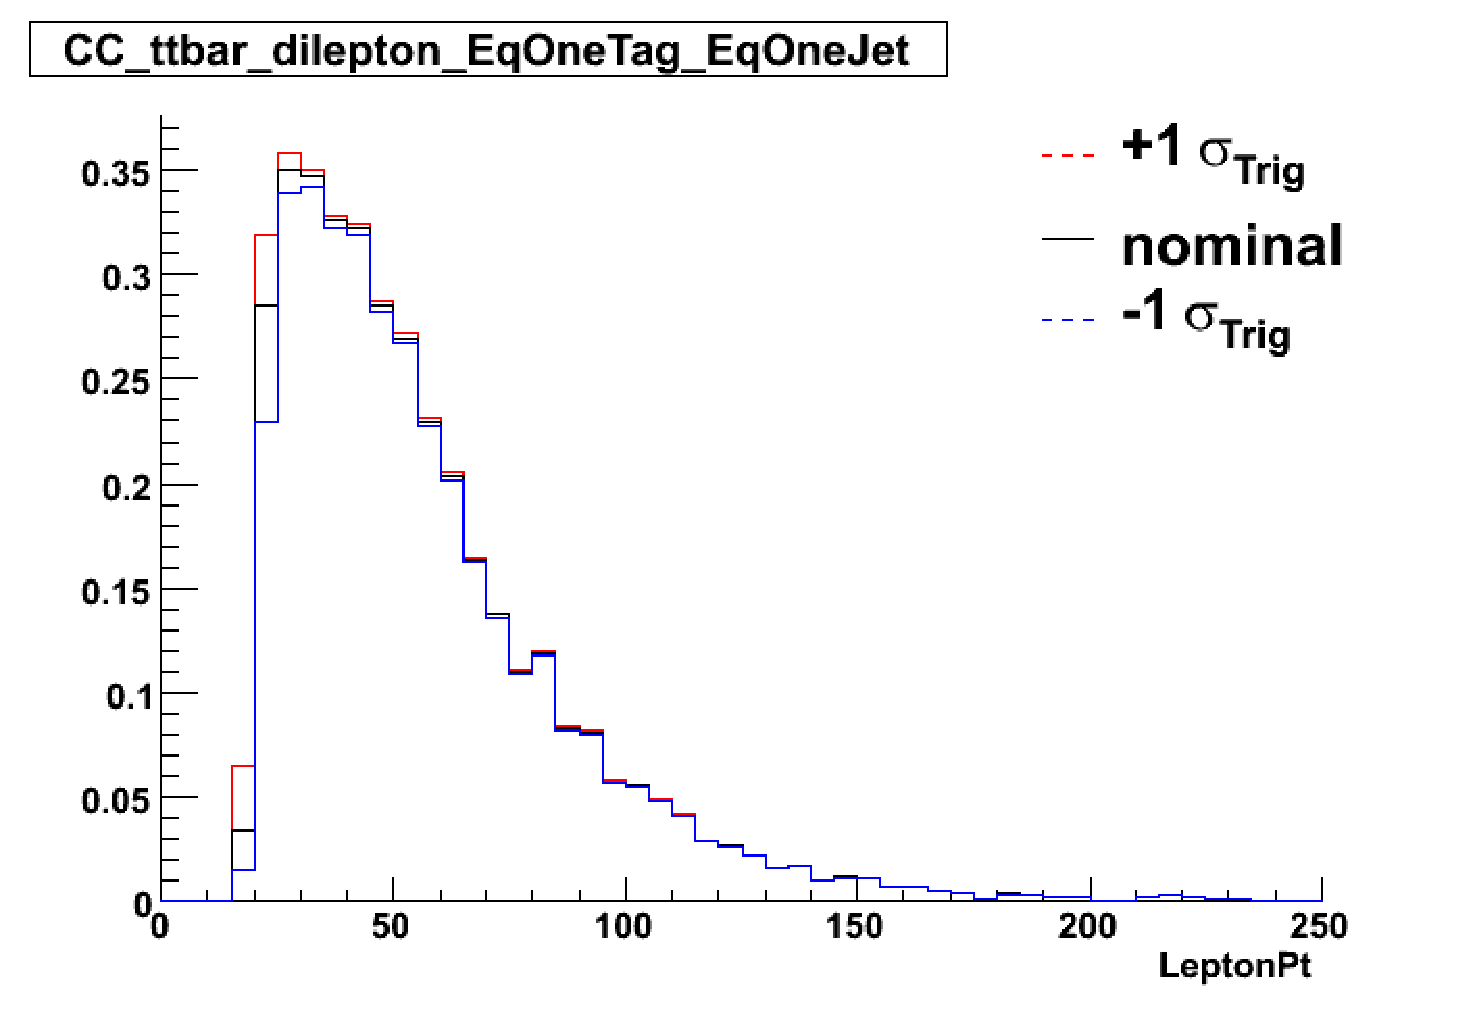
\includegraphics[width=0.75\textwidth]{eps/Systematics/trigger.eps}
\end{center}
\vspace{-0.1in}
\caption{Electron $p_{T}$ in weighted $\dilepton$ Monte Carlo events. The three curves represent the estimated yield in each $p_{T}$ bin for the case of $+1\sigma$ trigger weights (red), nominal trigger weights (black), and $-1\sigma$ trigger weights (blue).}
\label{triggeruncer}
\end{figure}

\item {\bf Primary vertex selection efficiency} \\
The longitudinal position of the primary interaction vertex is not well modeled in the Monte Carlo. The maximum deviation between the data and Monte Carlo is $3\%$ thus this number was taken as the systematic uncertainty. This uncertainty accounts for the beam profile along the longitudinal direction~\cite{beamshifts}.

\item {\bf Jet reconstruction and identification} \\
This systematic is due to the difference between the data and Monte Carlo for the $\eta$ and number of jets distributions. A $2\%$ uncertainty is assigned to this effect.

\item {\bf Jet energy scale (JES) and jet energy resolution} \\
The JES correction is raised and lowered by one standard deviation and
the whole analysis is repeated. In the data the JES uncertainty
contains the jet energy resolution uncertainty; however, in the Monte Carlo
the jet energy resolution uncertainty is not taken into account in the
JES uncertainty. To account for this the Monte Carlo energy smearing
is varied by the size of the jet energy resolution in MC. This
uncertainty affects the acceptance and the shapes of the
distributions. The $1\sigma$ error on the JES as a function of jet $p_{T}$ for central jets is shown in Fig.~\ref{jes2}. The JES uncertainty is larger for lower $p_{T}$ and more forward jets.

\begin{figure}[!h!tbp]
\begin{center}
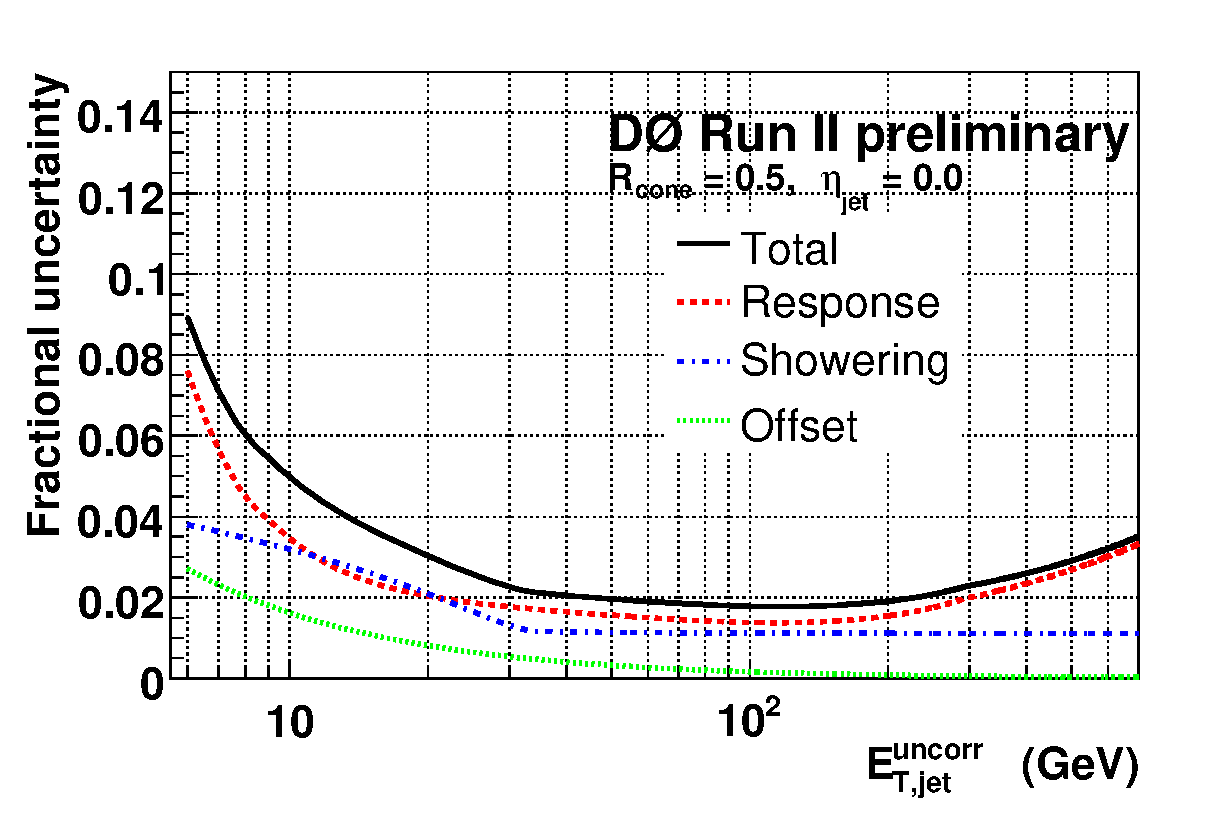
\includegraphics[width=0.75\textwidth]{eps/Systematics/jes.eps}
\end{center}
\vspace{-0.1in}
\caption{$1\sigma$~uncertainties from each of the jet energy scale components as a function of jet $p_{T}$ for jets with $\eta=0.0$. The total uncertainty is shown by the black line. }
\label{jes2}
\end{figure}

\item {\bf Jet fragmentation} \\
The uncertainty of the jet fragmentation model is determined by the difference in fragmentation models between the Pythia and Herwig Monte Carlo generators. This uncertainty also covers the uncertainties due to initial and final state radiation. The total uncertainty is $5\%$ for $\dilepton$ and single top quark events and $7\%$ for $\lepjets$~events.

\item {\bf Electron reconstruction and identification efficiency} \\
This uncertainty derives from the error on the electron reconstruction Monte Carlo correction factor. The uncertainty is determined by varying the correction factor by $1\sigma$ in the parameterized bins of $p_{T}$ and $\phi$. The total uncertainty is determined to be $2\%$.

\item {\bf Electron track matching and likelihood efficiency} \\
This uncertainty derives from the error on the electron track match and likelihood Monte Carlo correction factor. The uncertainty is determined by varying the correction factor by $1\sigma$ in the parameterized bins of $\eta$ and $\phi$. The total uncertainty is determined to be $5\%$.

\item {\bf Muon reconstruction and identification efficiency} \\
This uncertainty derives from the error on the muon reconstruction Monte Carlo correction factor. The uncertainty is determined by varying the correction factor by $1\sigma$ in the parameterized bins of $\eta$ and $\phi$. The total uncertainty is determined to be $7\%$.

\item {\bf Muon track matching and isolation} \\
This uncertainty derives from the error on the muon track match and isolation Monte Carlo correction factor. The uncertainty is determined by varying the correction factor by $1\sigma$ in the parameterized bins of $\eta$ and $\phi$ for the track match factor and $p_{T}$ and the number of jets for the isolation factor. The total uncertainty is determined to be $2\%$.

\item {\bf Matrix method normalization} \\
The normalization of the W+jets and multijet backgrounds is performed using the matrix method and its error is dominated by the error on the efficiency that a lepton not originating from a $W$ decay will pass the electron likelihood or muon isolation cut ($\delta\varepsilon_{\rm{Multijet}}$). The statistics of the normalized samples also contributes to the total uncertainty. The average values and errors for $\varepsilon_{\rm{Multijet}}$ for both electron and muon events is shown in Table~\ref{eps-qcd}.

\begin{table}[!h!tbp]
\begin{center}
\caption{$\varepsilon_{\rm{Multijet}}$ for electrons as a function of
the trigger period and jet multiplicity, and $\varepsilon_{\rm{Multijet}}$ for muons averaged over $\eta$. The definition of the trigger periods is found in Chapter~\ref{analysis}.}
\label{eps-qcd}
\begin{tabular}{c|ccccc|c}
%\multicolumn{7}{c}{\hspace{0.8in}\underline{Fake-Lepton Probabilities}}
%\vspace{0.05in}\\
& \multicolumn{5}{c|}{ Electron $\varepsilon_{\rm{Multijet}}$ For Five Trigger Periods ($\%$)} & \multicolumn{1}{c}{ Muon $\varepsilon_{\rm{Multijet}}$  ($\%$)} \\
Jets & I   &     II     &     III    &     IV    &     IV     &     I \\
\hline 
 2 & $12.8 \pm 1.0$ & $19.2 \pm 1.0$ & $18.8 \pm 2.2$ & $19.4 \pm 1.1$ & $22.0 \pm 1.2$ & $35.8 \pm 3.2$ \\
 3 & $13.6 \pm 1.5$ & $19.5 \pm 1.6$ & $19.8 \pm 3.4$ & $19.2 \pm 1.6$ & $19.4 \pm 1.7$ & $34.2 \pm 4.5$ \\
\end{tabular}
\vspace{-0.1in}
\end{center}
\end{table}


\item {\bf Ratio of $Wb\bar{b}+Wc\bar{c}$ to $Wjj$ Events} \\
There is a $30\%$ systematic error due to the uncertainty on this ratio. The error is much larger than the fit to the events in the zero tag sample to account for theoretical shape-dependent errors that are not modeled in the Monte Carlo. The largest of these theoretical errors is the shape change to the $b$-quark $p_{T}$ between NLO and LO $Wbb$ events. The error on this ratio is folded into the overall matrix method normalization uncertainty when determining the acceptance and background yield uncertainties.

\item {\bf Monte Carlo tag-rate functions}\\
The uncertainty associated with the tag-rate functions is evaluated by shifting the TRFs by $\pm1\sigma$ and evalulating the change in the signal acceptance and background yield. The tag-rate function uncertainties are dominated by the assumed fraction of heavy flavor in the multijet samples used to determine the fake tagging rate in data and the decreased statistics in each bin due the parameterization in $p_{T}$ and $\eta$. The tag rate functions for $B$-jets and charm-jets and the $1\sigma$~error bands are shown in Fig.~\ref{trfserror2}. The total uncertainty depends heavily on the number of $B$-tagged jets in the event.


\begin{figure}[!h!tbp]
\begin{center}
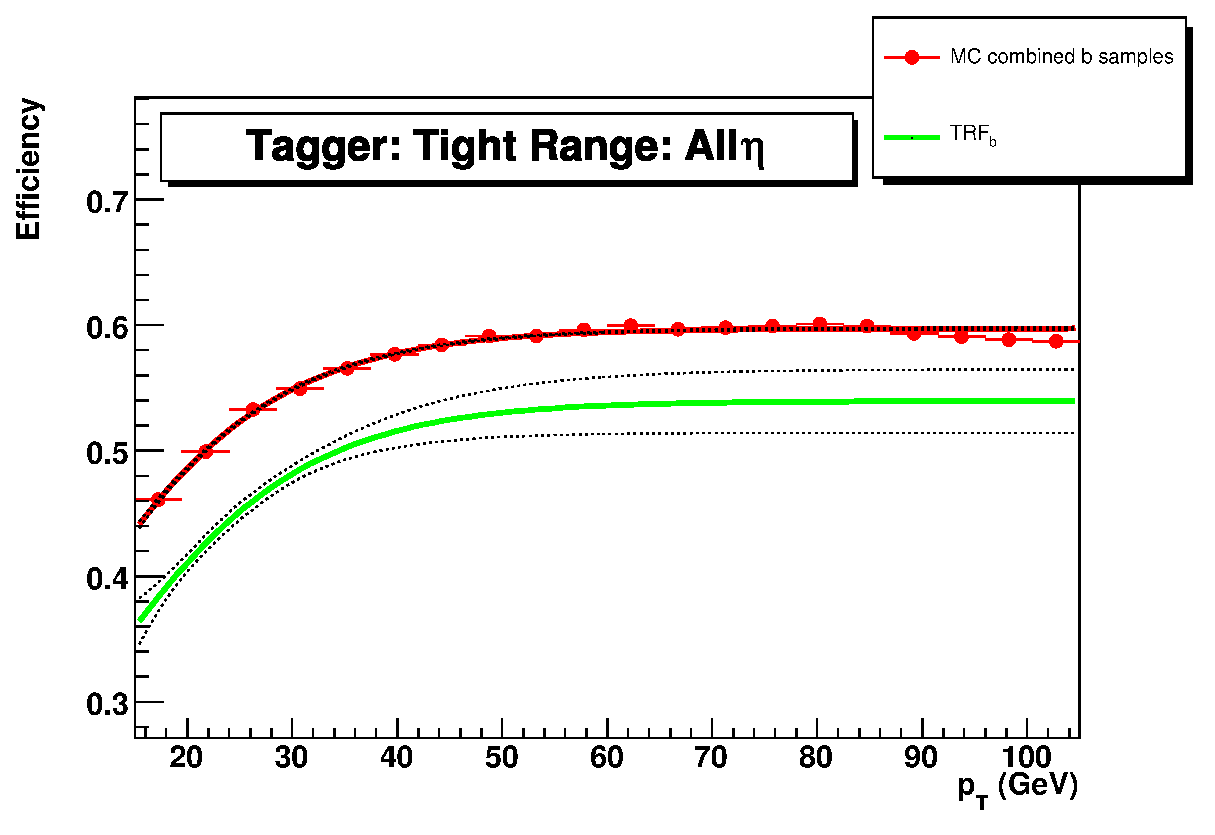
\includegraphics[width=0.48\textwidth]{eps/Systematics/trf_b_0.775_pt.eps}
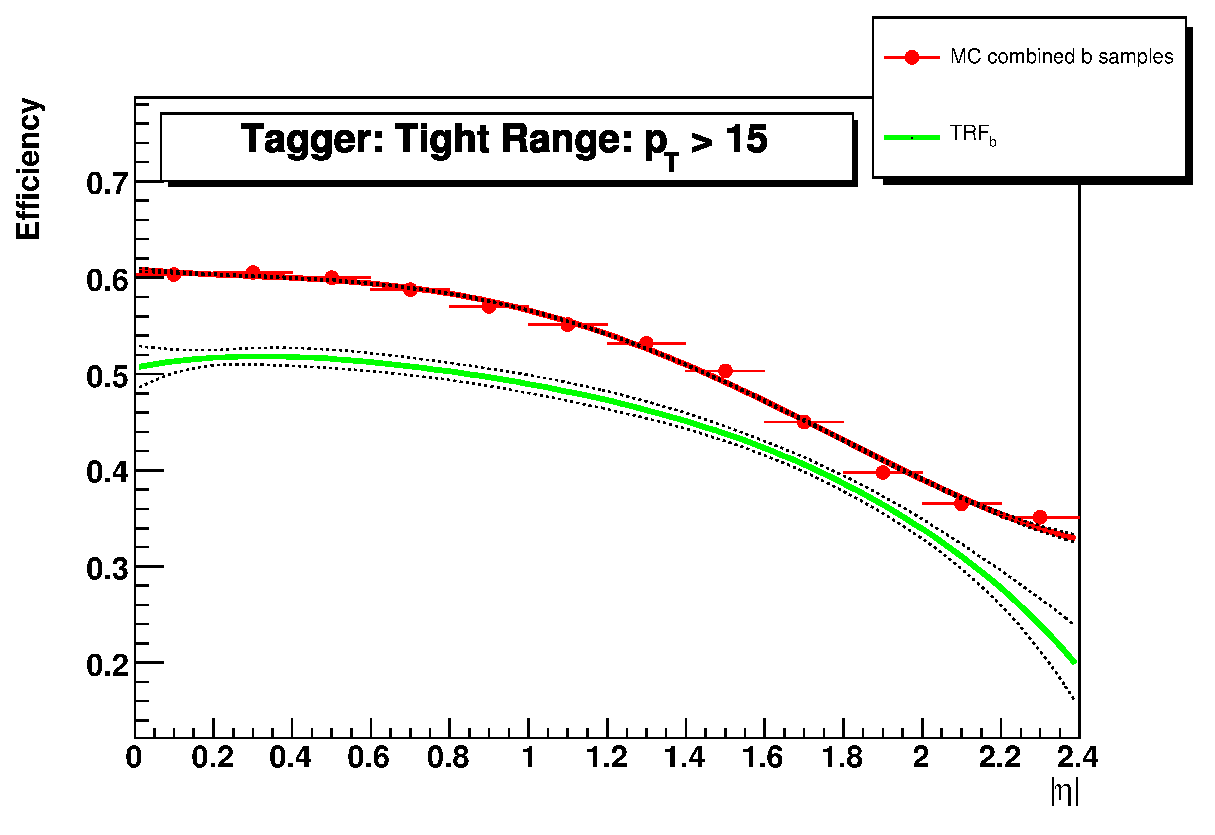
\includegraphics[width=0.48\textwidth]{eps/Systematics/trf_b_0.775_eta.eps}
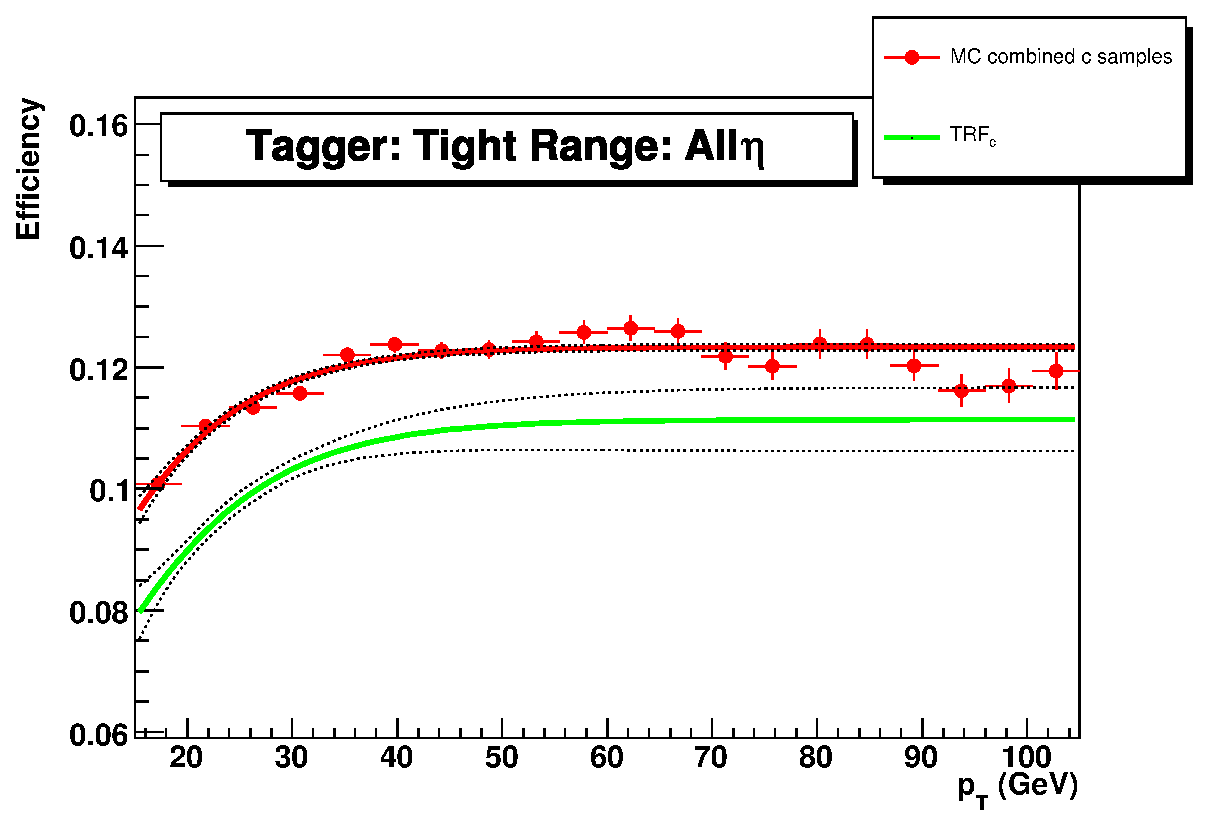
\includegraphics[width=0.48\textwidth]{eps/Systematics/trf_c_0.775_pt.eps}
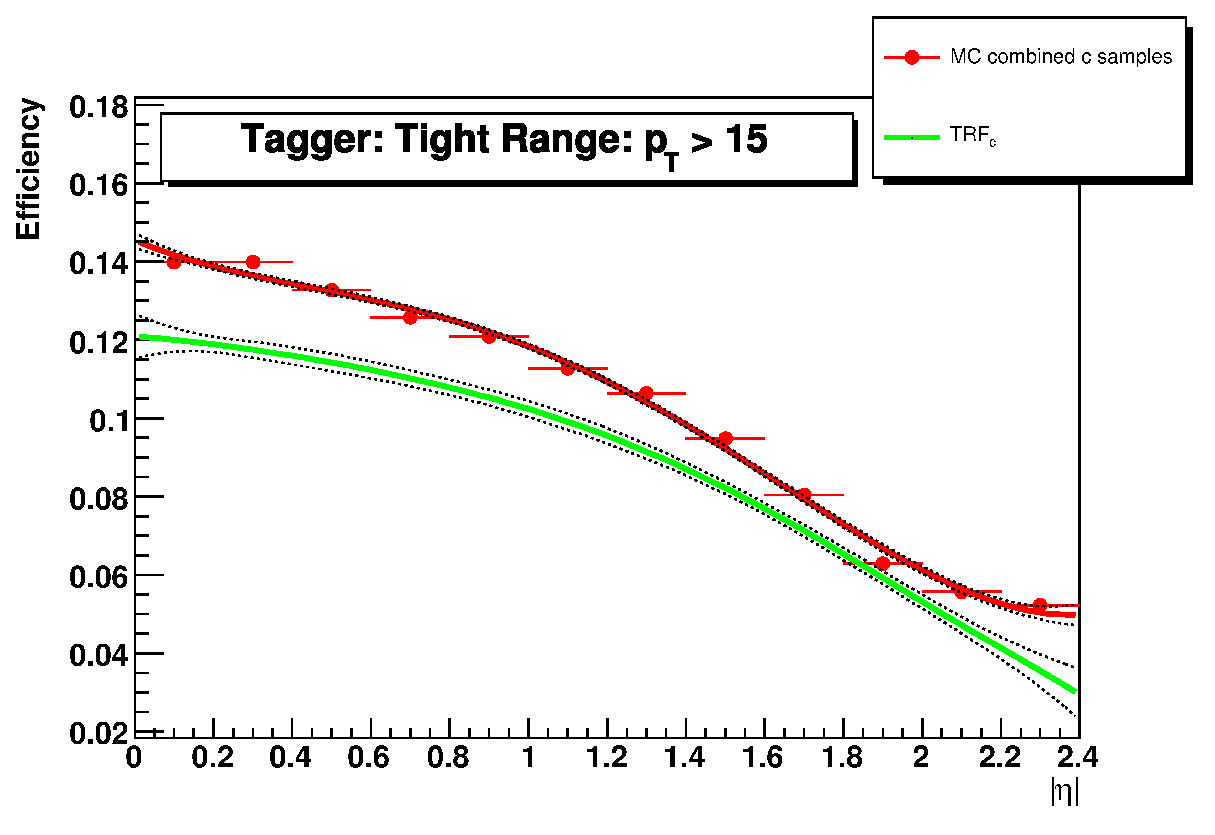
\includegraphics[width=0.48\textwidth]{eps/Systematics/trf_c_0.775_eta.eps}
\end{center}
\vspace{-0.1in}
\caption{Neural network $B$-jet tagger efficiency (green line) and $1\sigma$~error bands (dashed lines) jet $p_{T}$ and $\eta$ for $B$-jets (upper row) and charm-jets (lower row). The red lines represent the efficiency of the $B$-tagging algorithm when applied directly to the Monte Carlo.}
\label{trfserror2}
\end{figure}

\end{itemize}

\clearpage
\section{Ensemble Testing}
\label{ensembles}

Ensemble tests are performed to ensure there is no bias in the measured cross section. An ensemble is a group of pseudo-datasets created with a known fraction of signal and background events. Since the fractions are known the linearity of the measured cross section can be tested against the known cross section.

The ensembles are generated from a large set of weighted signal and background events. For each analysis channel the total background yield, as shown in Chapter~\ref{background}, is used as the expected value of a Poisson distribution and a new background yield is generated from this distribution. The uncertainty in the yield due to systematics is included when generating a new background and signal yield as explained in Appendix~\ref{ensemblegeneration}. This procedure will on average produce the expected background compositeness (e.g. ratio of Wbb to Wjj events). The cross section is then determined for all psuedo-datasets in the ensemble.

Five ensembles were generated with the following $s+t$-channel input signal cross sections:

\begin{itemize}
\item $\sigma_{s+t} = 2$~pb.
\item $\sigma_{s+t} = 2.9$~pb. (Expected Standard Model cross section)
\item $\sigma_{s+t} = 4$~pb.
\item $\sigma_{s+t} = 6$~pb.
\item $\sigma_{s+t} = 8$~pb.
\end{itemize}

\noindent 2,000 datasets were generated in each ensemble. A histogram of the measured cross sections for each of these ensembles is shown in Fig.~\ref{blue}. A plot of the mean of these histograms versus the input cross section is shown in Fig.~\ref{linearity}. A linear fit to the data points yields a good $\chi^{2}$/dof of 0.13/3, a slope consistent with 1 of $1.03\pm0.03$, and an offset of $0.32\pm0.09$.

\begin{figure}[!h!tbp]
\begin{center}
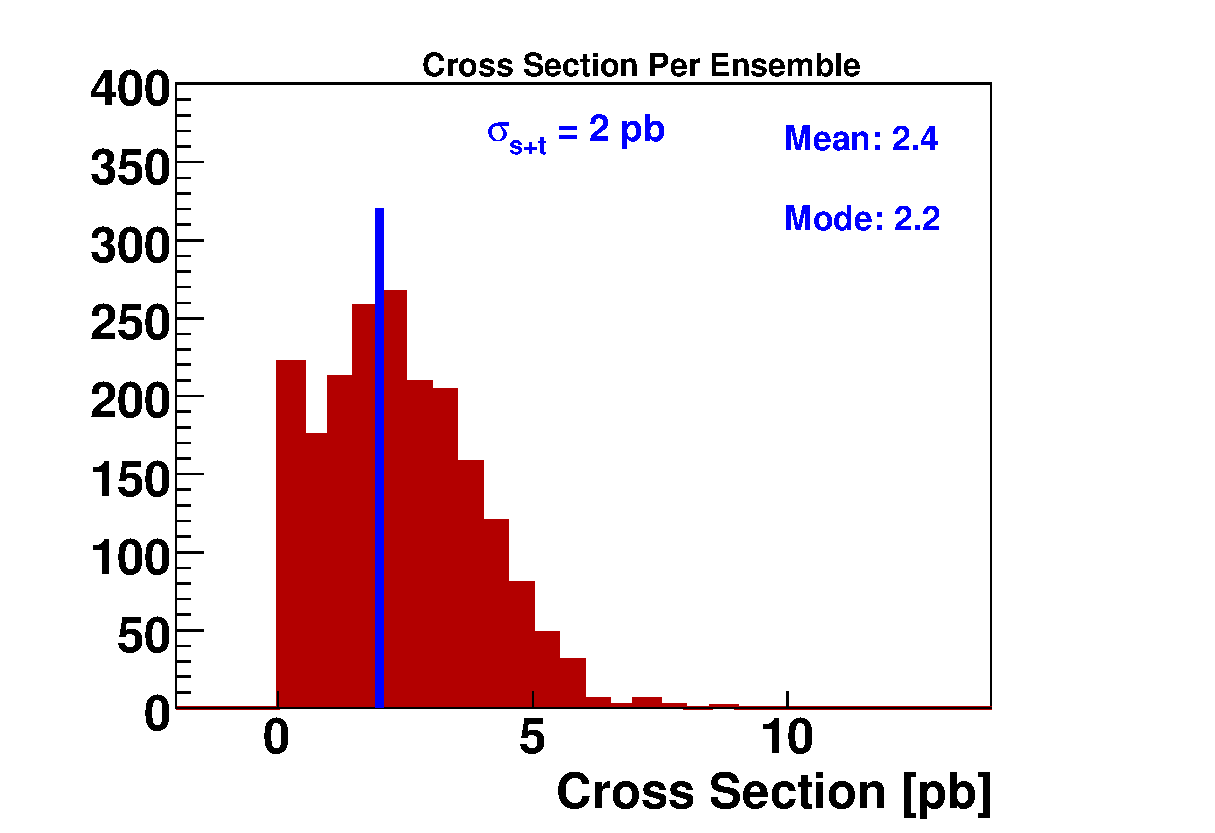
\includegraphics[width=0.48\textwidth]{eps/Limits/Blue2.0.eps}
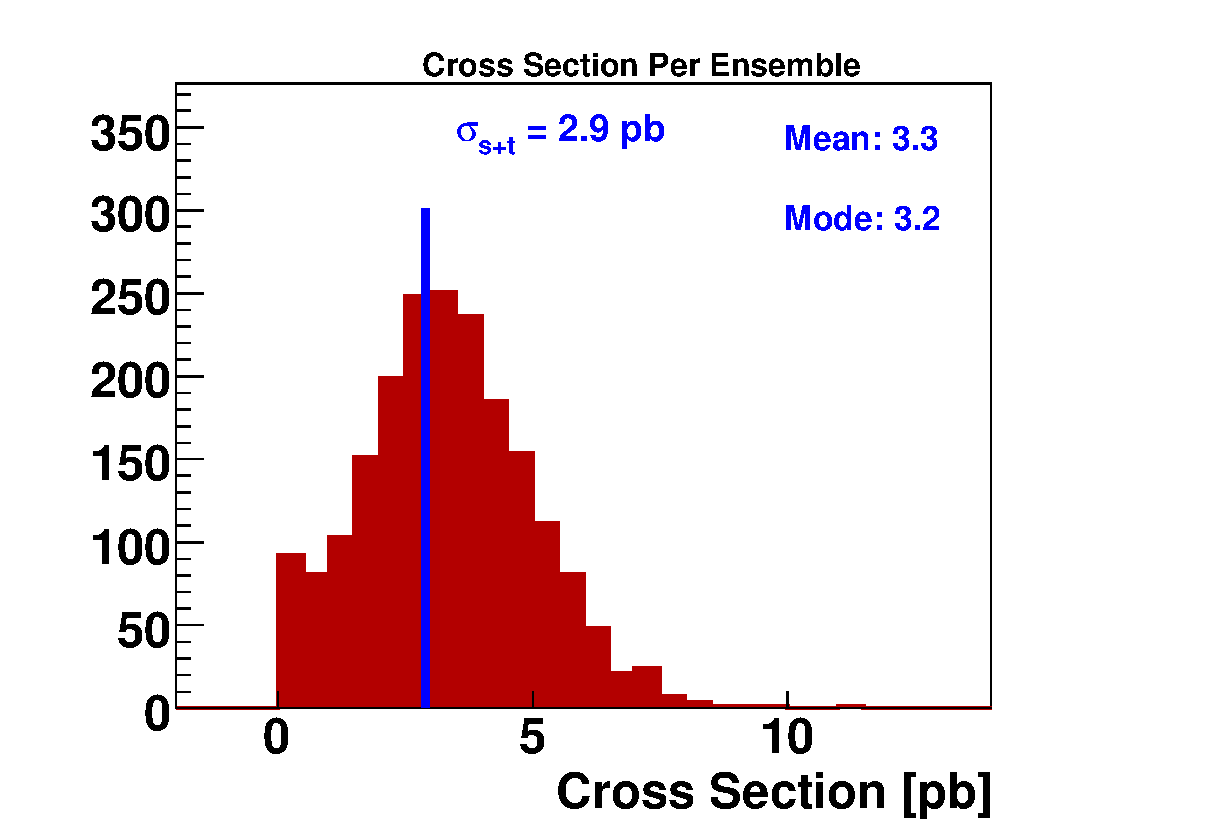
\includegraphics[width=0.48\textwidth]{eps/Limits/Blue2.9.eps}
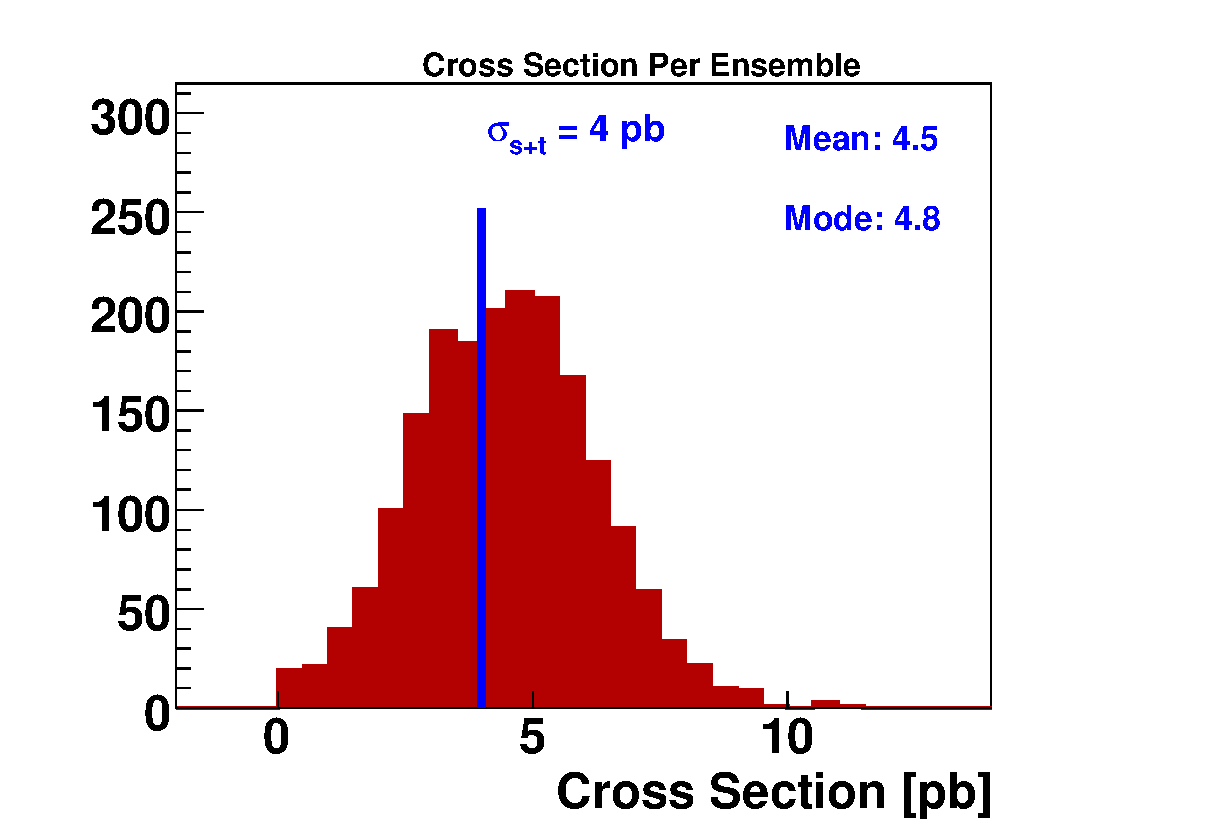
\includegraphics[width=0.48\textwidth]{eps/Limits/Blue4.0.eps}
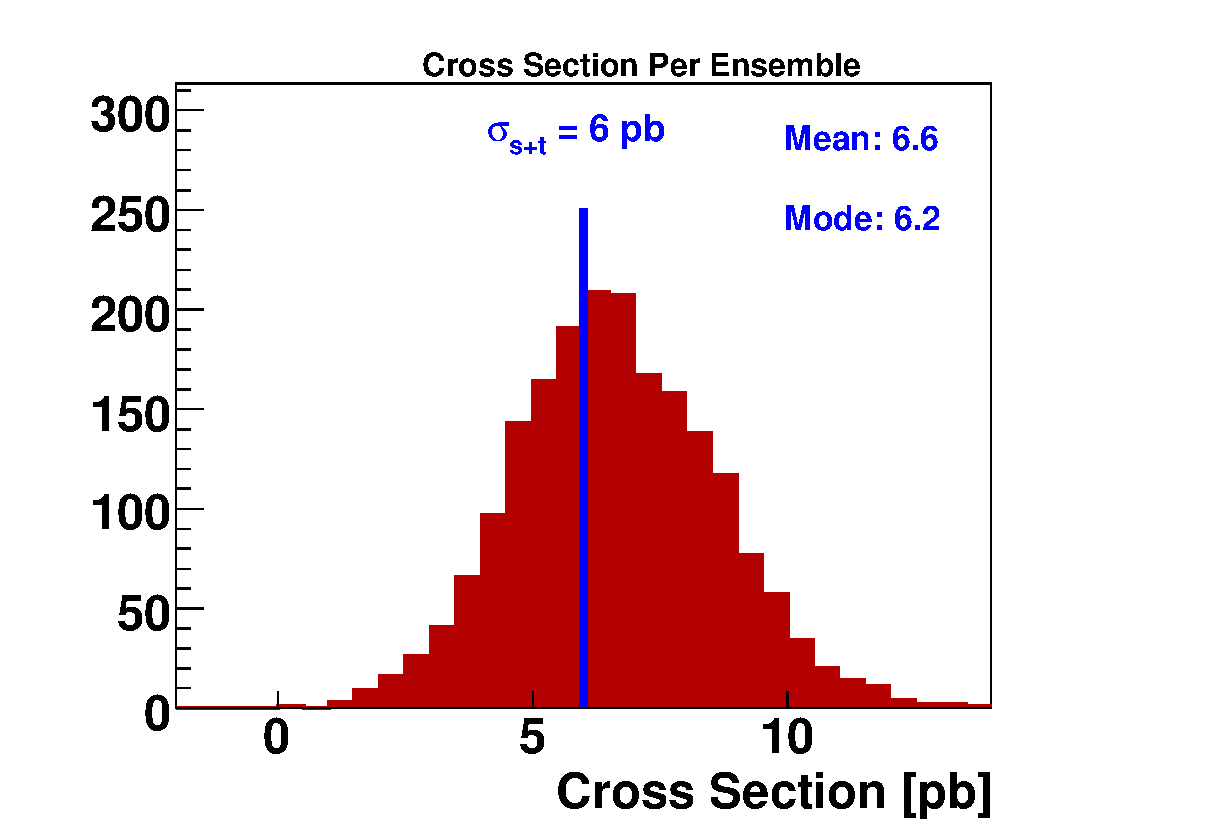
\includegraphics[width=0.48\textwidth]{eps/Limits/Blue6.0.eps}
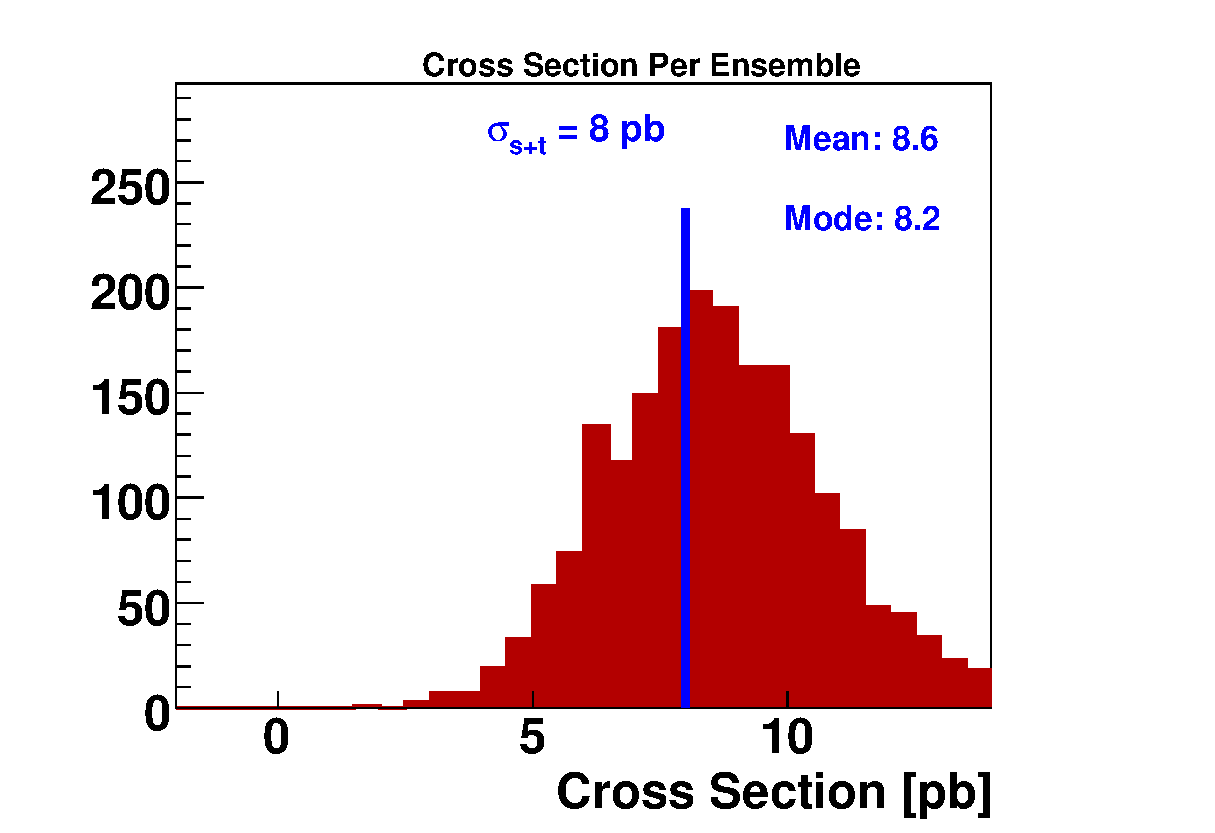
\includegraphics[width=0.48\textwidth]{eps/Limits/Blue8.0.eps}
\end{center}
\vspace{-0.1in}
\caption{Observed cross section for a set of 2,000 pseudo-datasets for the five ensembles: $\sigma_{s+t}=2.0$~pb (upper left), $\sigma_{s+t}=2.9$~pb (upper right), $\sigma_{s+t}=4.0$~pb (middle left), $\sigma_{s+t}=6.0$~pb (middle right), and $\sigma_{s+t}=8.0$~pb (bottom middle)}
\label{blue}
\end{figure}


\begin{figure}[!h!tbp]
\begin{center}
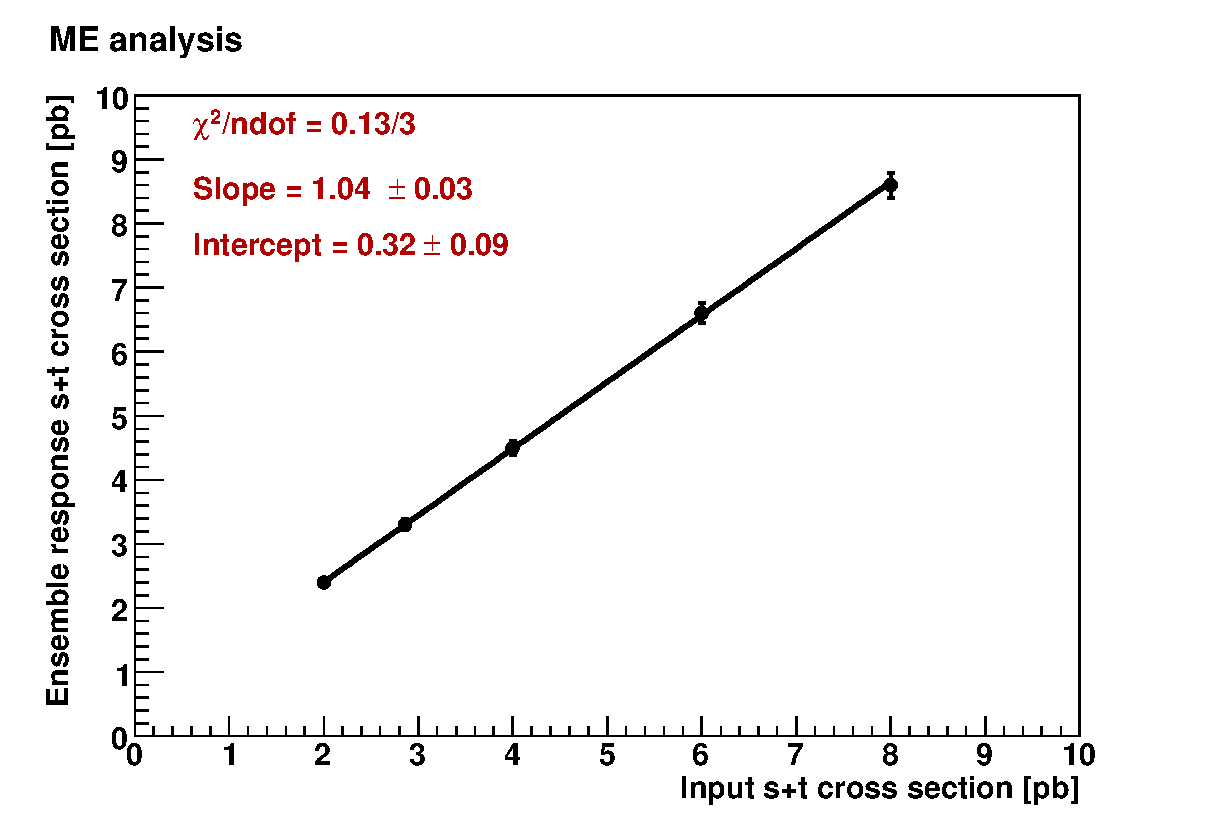
\includegraphics[width=0.75\textwidth]{eps/Limits/Linearity.eps}
\end{center}
\vspace{-0.1in}
\caption{Response of the five generated ensemble sets versus input cross section. The response is measured as the mean value of the histogram for each ensemble.}
\label{linearity}
\end{figure}

\clearpage
\section{Expected Results}
\label{exp-performance}

This section presents the expected performance of the analysis given a Standard Model single top signal. To test the expected sensitivity the number of data events is set equal to the number of signal and background events in each bin of the Likelihood (i.e. the excess of data over background in each bin is equal, by construction, to the number of events expected from a signal with $\sigma=2.9$ pb). This test is performed for each analysis channel and various combinations of the channels. Figs.~\ref{exp-post-1d-2j} and \ref{exp-post-1d-3j} show the
resulting $tb$+$tqb$\footnote{$tb+tqb$ is used to donate the combined $s$-channel plus $t$-channel cross section measurement} posterior for the combined $e$+$\mu$ $\geq$~1
$B$-tag channel in two-jet and three-jet events.
Figure~\ref{exp-post-1d-allj} shows the $tb$+$tqb$ posterior for the
combination of all channels. The figures on the left correspond to the case
of only statistical uncertainties, whereas the figures on the right include statistical and systematic uncertainties. 

\vspace{0.1in}
\begin{figure}[!h!tbp]
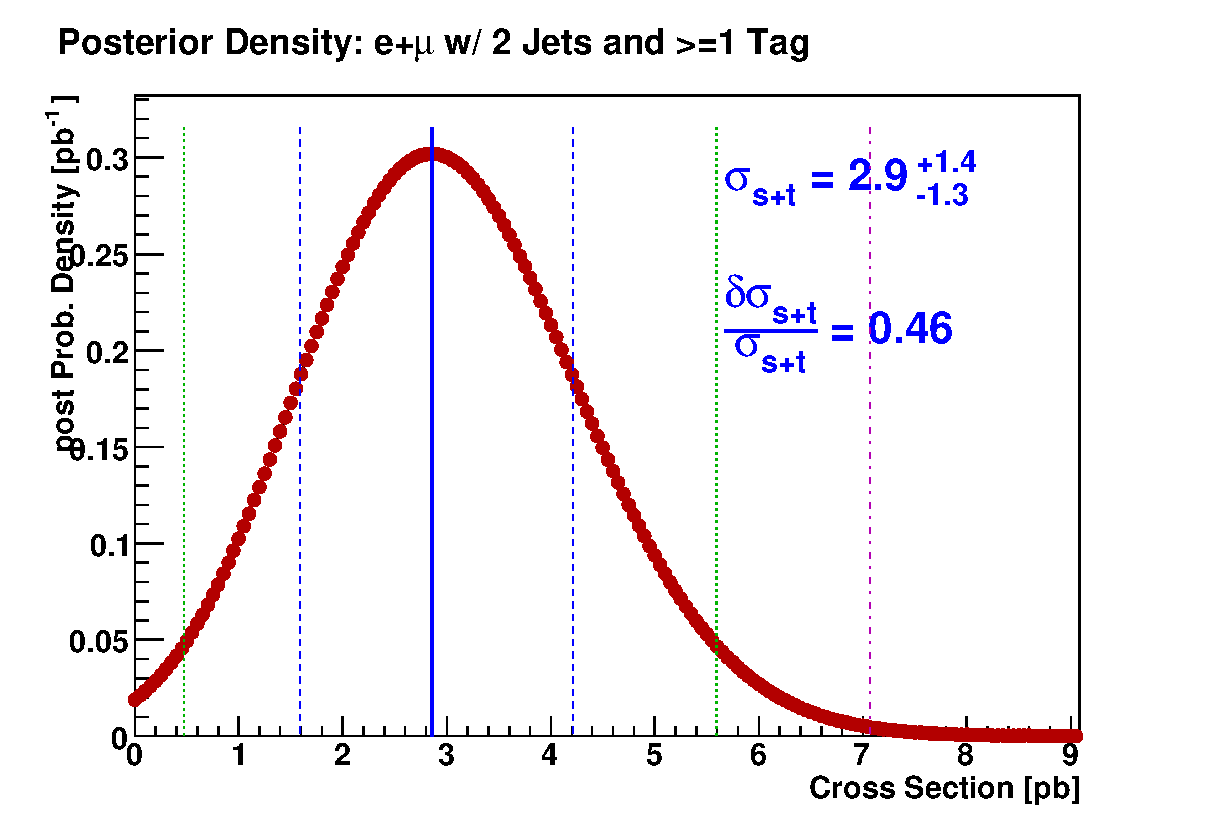
\includegraphics[width=0.49\textwidth]
{eps/MatrixElement/posterior/nosys/expected_limit_TBTQ_LeptonsCombined_2Jet_TagsCombined}
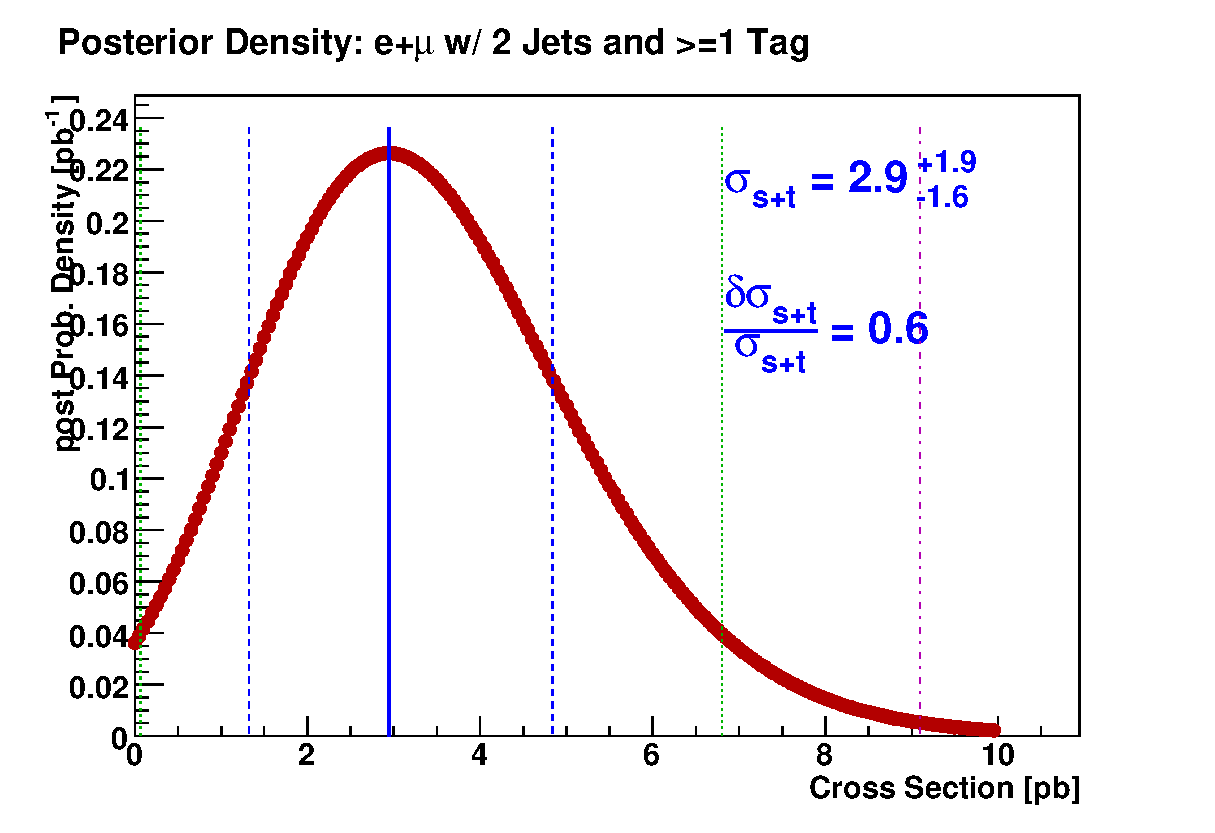
\includegraphics[width=0.49\textwidth]
{eps/MatrixElement/posterior/sys/expected_limit_TBTQ_LeptonsCombined_2Jet_TagsCombined}
\vspace{-0.1in}
\caption{Expected 1D posterior plots for the combined
$e$+$\mu$ $\geq$~1 $B$-tag channel in two-jet events, with statistical
uncertainties only (left plot) and including also systematic
uncertainties (right plot).}
\label{exp-post-1d-2j}
\end{figure}

\vspace{0.1in}
\begin{figure}[!h!tbp]
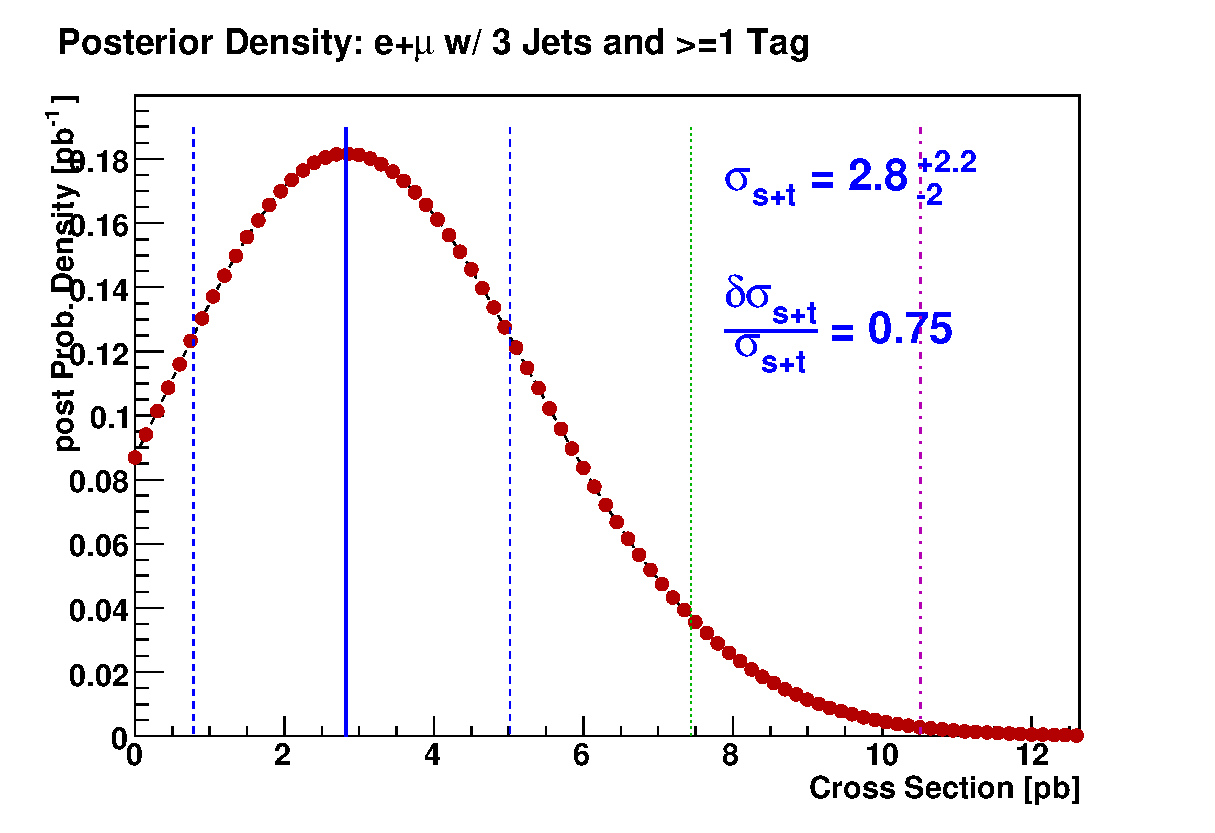
\includegraphics[width=0.49\textwidth]
{eps/MatrixElement/posterior/nosys/expected_limit_TBTQ_LeptonsCombined_3Jet_TagsCombined}
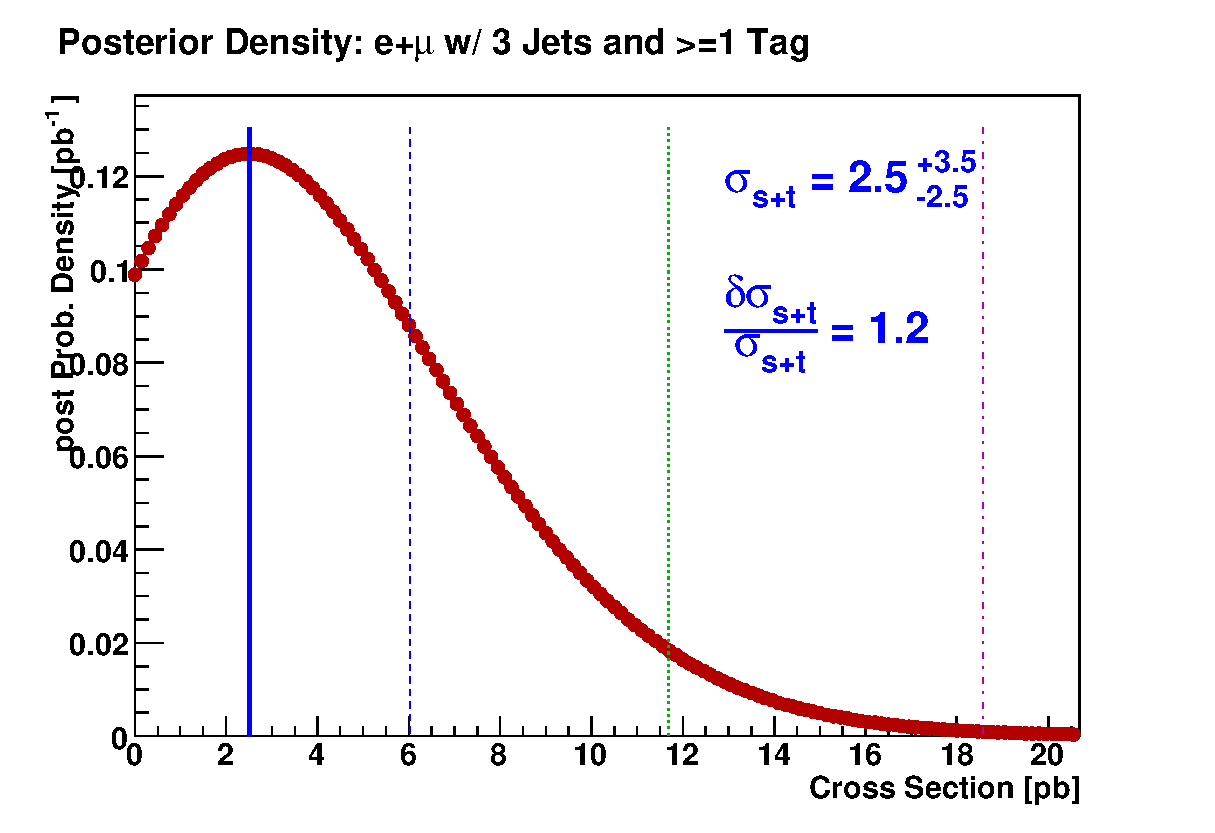
\includegraphics[width=0.49\textwidth]
{eps/MatrixElement/posterior/sys/expected_limit_TBTQ_LeptonsCombined_3Jet_TagsCombined}
\vspace{-0.1in}
\caption{Expected 1D posterior plots for the combined
$e$+$\mu$ $\geq$~1 $b$-tag channel in three-jet events, with
statistical uncertainties only (left plot) and including also
systematic uncertainties (right plot).}
\label{exp-post-1d-3j}
\end{figure}

\vspace{0.1in}
\begin{figure}[!h!tbp]
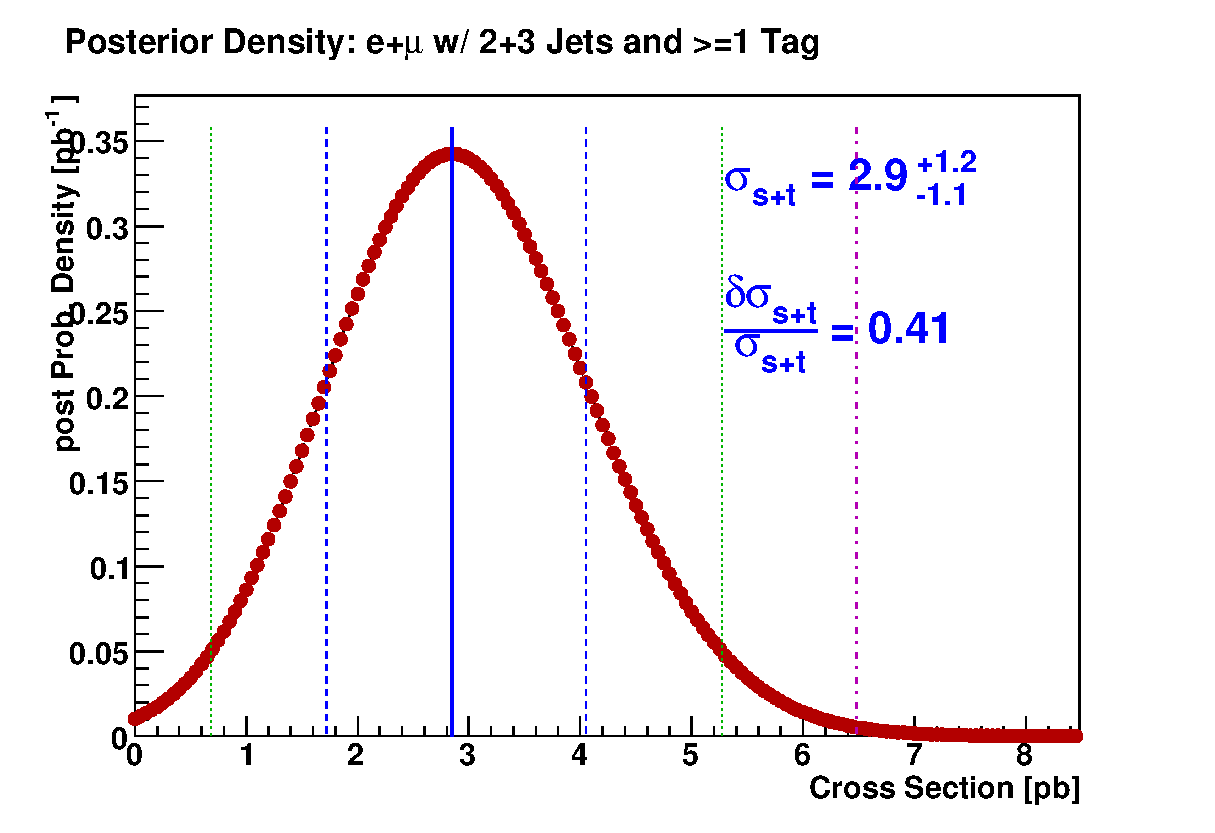
\includegraphics[width=0.49\textwidth]
{eps/MatrixElement/posterior/nosys/expected_limit_TBTQ_LeptonsCombined_JetsCombined_TagsCombined}
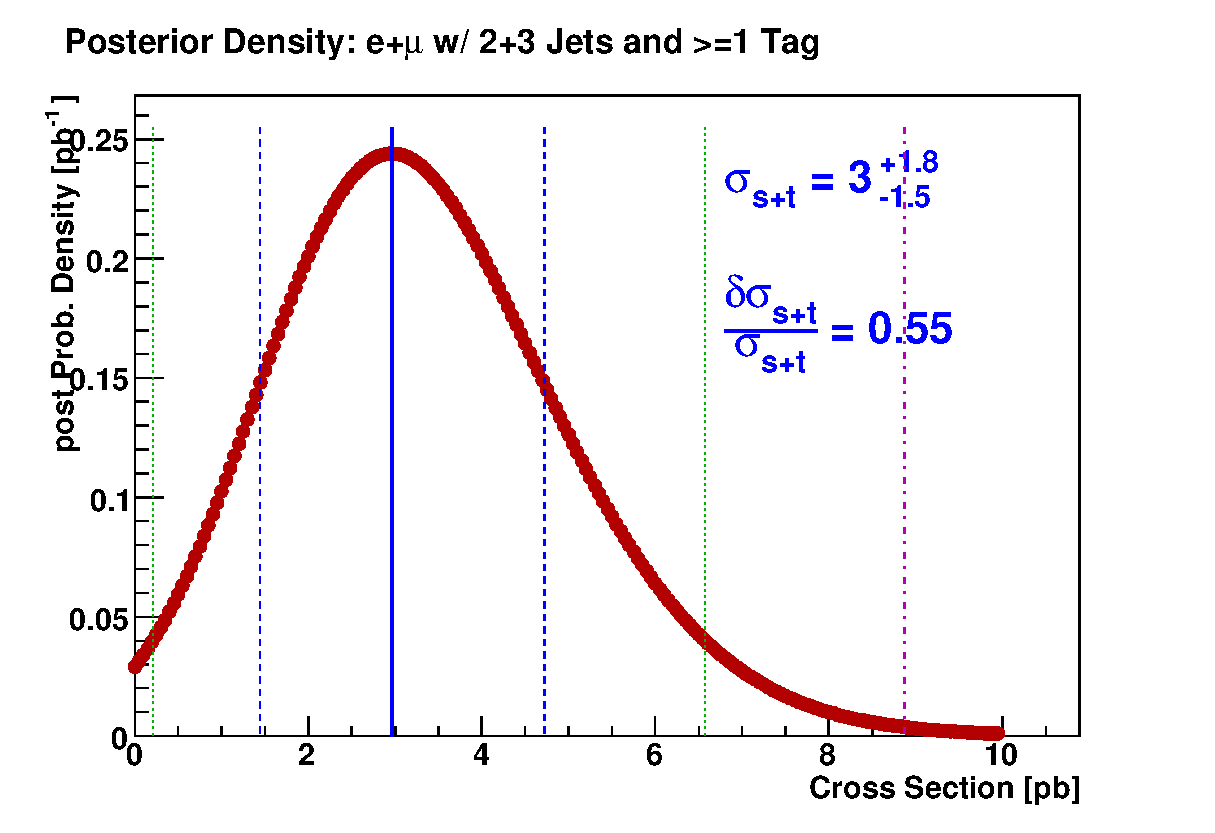
\includegraphics[width=0.49\textwidth]
{eps/MatrixElement/posterior/sys/expected_limit_TBTQ_LeptonsCombined_JetsCombined_TagsCombined}
\vspace{-0.1in}
\caption{Expected 1D posterior plots for the
combination of all channels, with statistical uncertainties only (left
plot) and including also systematic uncertainties (right plot).}
\label{exp-post-1d-allj}
\end{figure}

Table~\ref{tab:expxsecs} shows the expected cross sections for various
combinations of analysis channels. The expected result for each
combination is consistent with the standard model cross
section. Table~\ref{exp-errors} summarizes the relative uncertainty on
the expected $tb$+$tqb$ cross section measurement, defined as half the
width of the $tb$+$tqb$ posterior, divided by the cross section value
at the posterior peak.

\begin{table}[!h!tbp]
\begin{center}
\caption{Expected $tb$+$tqb$ cross sections, without and
with systematic uncertainties, for many combinations of the analysis
channels. The final expected result of this analysis are shown in the
lower right hand corner in bold type.}
\label{tab:expxsecs}
\begin{tabular}{c|cc|cc|cc|c}
%  \multicolumn{8}{c}{\hspace{0.5in}\underline{Expected $tb$+$tqb$ Cross Section}}\vspace{0.1in}\\
& \multicolumn{2}{c|}{1,2tags + 2,3jets}& \multicolumn{2}{c|}{$e$,$\mu$ + 2,3jets}
& \multicolumn{2}{c|}{$e$,$\mu$ + 1,2tags}& All \\
                 &  $e$-chan & $\mu$-chan& 1 tag & 2 tags& 2 jets& 3 jets&channels\\
\hline
Statistics only  &  $2.8^{+1.5}_{-1.4}$  & $2.8^{+1.8}_{-1.7}$ & $2.9^{+1.3}_{-1.2}$ & $2.8^{+2.5}_{-2.2}$ & $2.9^{+1.4}_{-1.3}$ & $2.8^{+2.2}_{-2.1}$ & $2.9^{+1.2}_{-1.1}$ \\
With systematics &  $3.0^{+2.2}_{-1.8}$  & $3.1^{+2.5}_{-2.1}$ & $2.9^{+1.8}_{-1.6}$ & $2.7^{+3.4}_{-2.7}$ & $2.9^{+1.9}_{-1.6}$ & $2.5^{+3.5}_{-2.5}$ & $\mathbf{3.0^{+1.8}_{-1.5}}$ \\
\end{tabular}
\vspace{-0.1in}
\end{center}
\end{table}

\vspace{-0.1in}
\begin{table}[!h!tbp]
\begin{center}
\caption{Relative uncertainties on the expected
$tb$+$tqb$ cross section, without and with systematic uncertainties,
for many combinations of the analysis channels. The best value from
all channels combined, with systematics, is shown in bold type.}
\label{exp-errors}
\begin{tabular}{l|cc|cc|cc|c}
%  \multicolumn{8}{c}{\hspace{0.5in}\underline{Relative Uncertainties on the Expected $tb$+$tqb$ Cross Section}}\vspace{0.1in}\\
& \multicolumn{2}{c|}{1,2tags + 2,3jets}& \multicolumn{2}{c|}{$e$,$\mu$ + 2,3jets}
& \multicolumn{2}{c|}{$e$,$\mu$ + 1,2tags}& All \\
                 &  $e$-chan & $\mu$-chan& 1 tag & 2 tags& 2 jets& 3 jets&channels\\
\hline
Statistics only  &  $52\%$  & $60\%$ & $45\%$ & $83\%$  &  $46\%$  & $75\%$  & $41\%$     \\
With systematics &  $67\%$  & $75\%$ & $59\%$ & $115\%$ &  $60\%$  & $121\%$ & $\mathbf{55\%}$     \\
\end{tabular}
\vspace{-0.1in}
\end{center}
\end{table}